\chapter{Protocol}
The following graph shows our experimental setup during the experiment.
To make this clear, the corresponding optical components have been marked.\\
\begin{figure}[h]
    \centering
    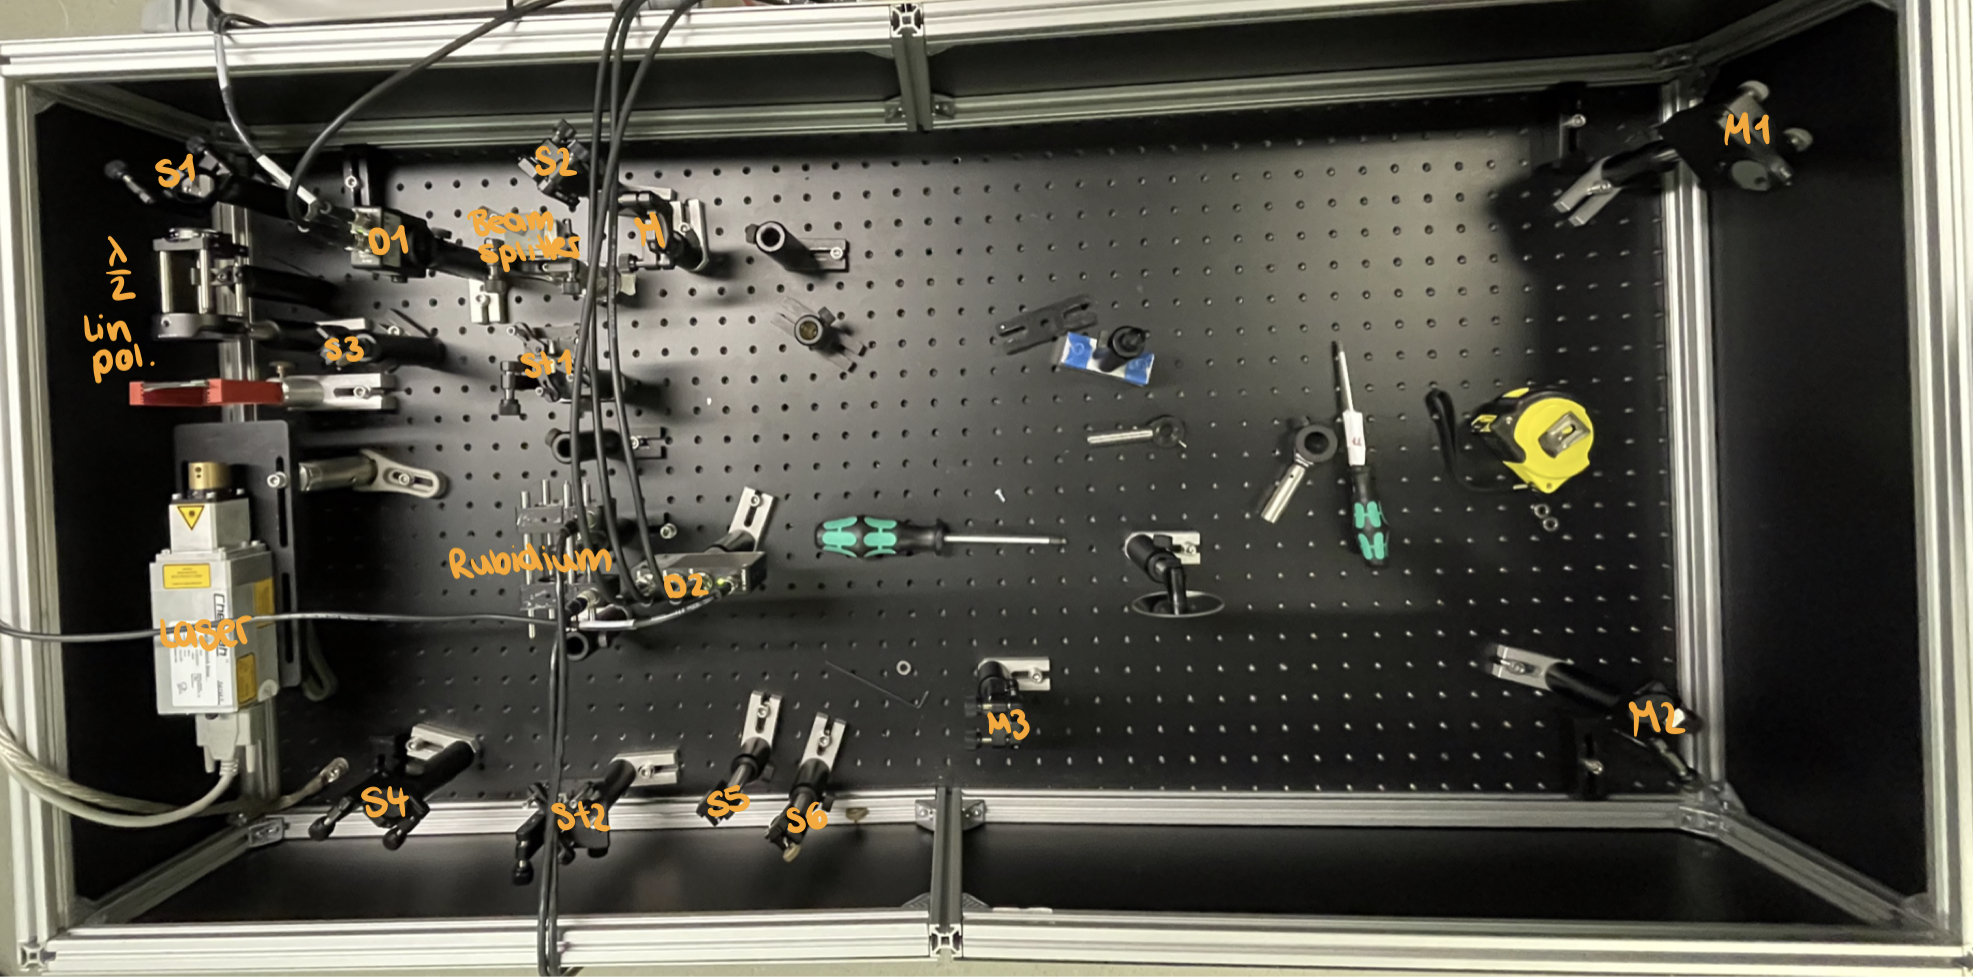
\includegraphics[scale=0.2]{Bilder/Versuch/Aufbau.jpg}
    \caption{Picture of the experimental setup}
   \end{figure}\\
As can be seen, the experimental setup
was constructed according to the diagram shown in the manual \ref{fig:anleitung}.\\
\begin{figure}[h]
    \centering
    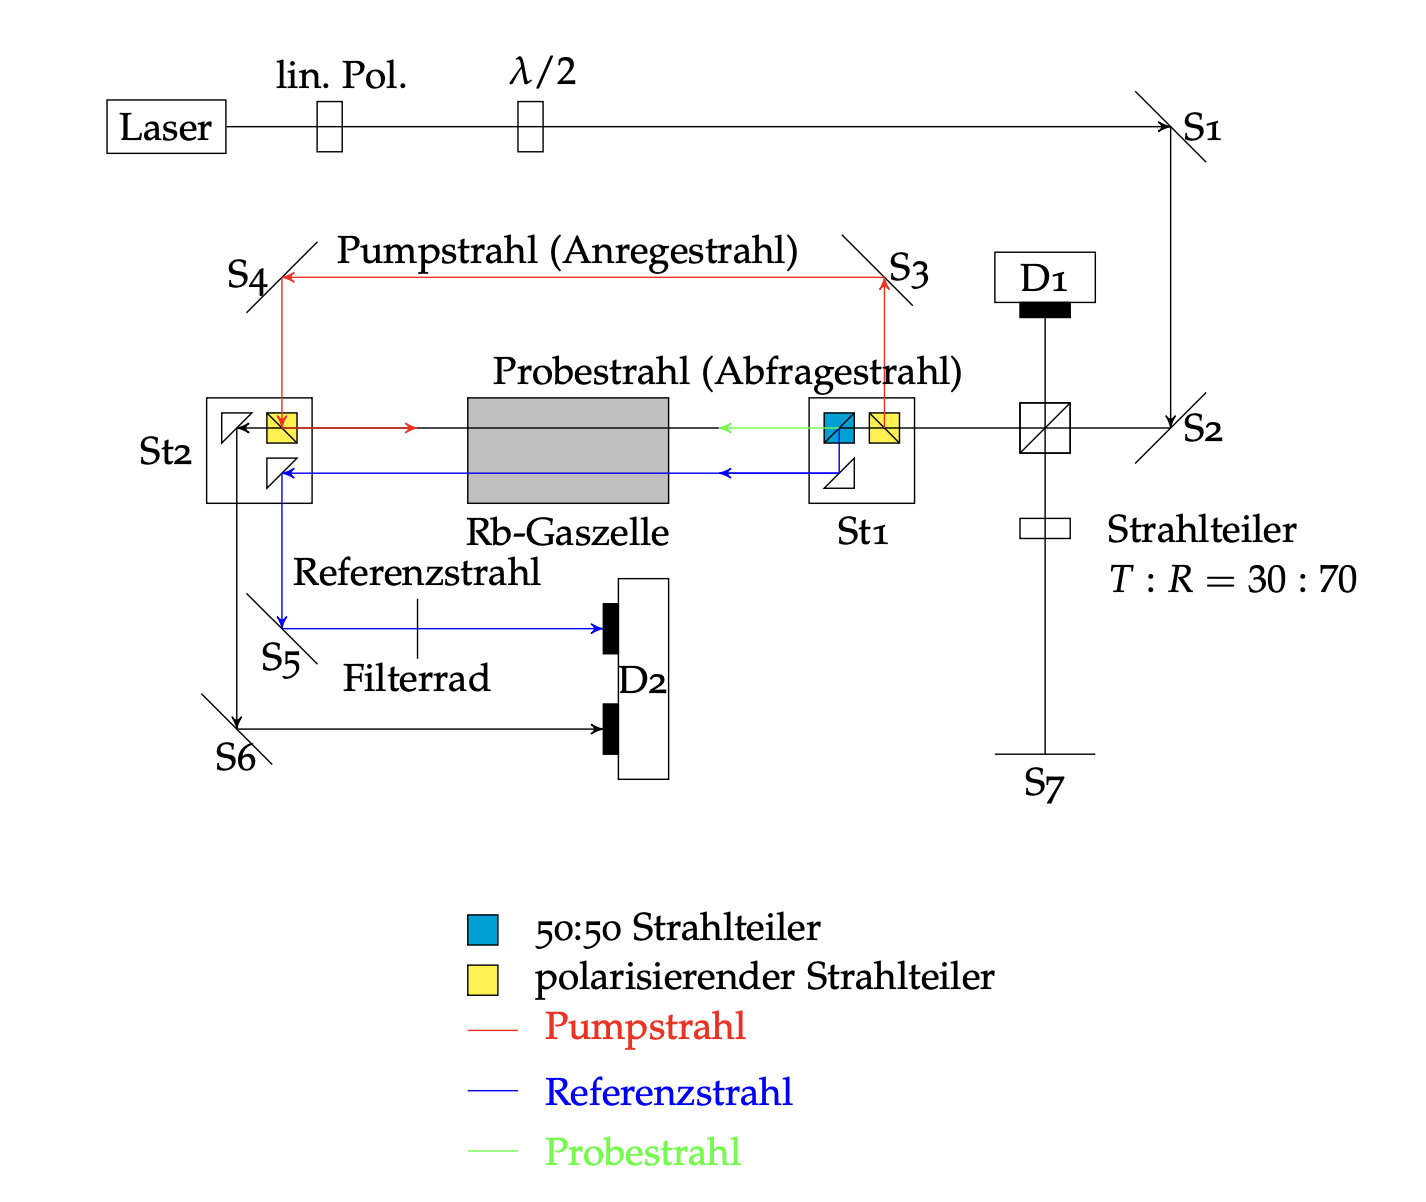
\includegraphics[scale=0.3]{Bilder/Versuch/Abbildung3.png}
    \caption{figure of the experimental setup from the instruction}
    \label{fig:anleitung}
   \end{figure}\\
Before measurement startet we build the set up after the manual and
then the different components i.e. the mirrors were aligned and adjusted according 
to the instructions.\\
After everything was adjusted we got used to the measuring program.\\
The different channels are defined as follows:\\
\begin{itemize}
    \item Channel 0 (Ai0): Diffrence
    \item Channel 1 (Ai1): Sample Beam
    \item Channel 2 (Ai2): /
    \item Channel 3 (Ai3): Reference Beam
    \item Channel 4 (Ai4): Fabry Perot Interferometer
    \item x-axis: laser current in mA
    \item y-axis: amplitude in V
\end{itemize}
During the experiment some distances were measured as well, those 
are illustrate in the follwing plot:\\
\begin{figure}[h]
    \centering
    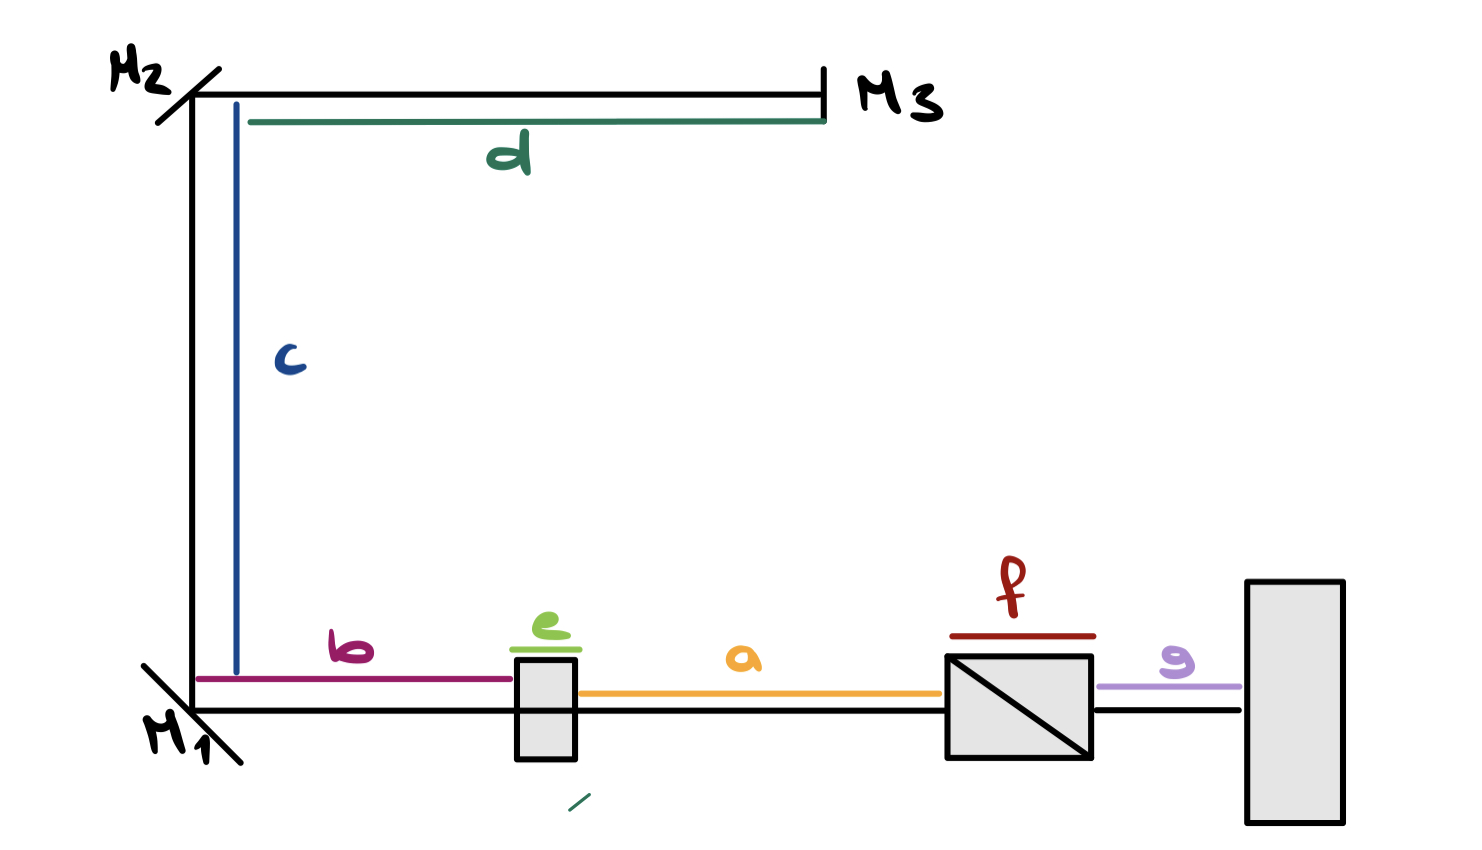
\includegraphics[scale=0.2]{Bilder/Versuch/langen.jpg}
   \end{figure}\\
The corersponding values are the followings:\
\begin{align}
    a &= (7.9 \pm 0,3)\,cm\\
    b &= (72.0 \pm 0,3)\,cm\\
    c &= (35.0 \pm 0,3)\,cm\\
    d &= (42.0 \pm 0,3)\,cm\\
    e &= (0.7 \pm 0,1)\,cm\\
    f &= (2.5 \pm 0,1)\,cm\\
    g &= (7.4 \pm 0,1)\,cm\\
\end{align}
The used measuring instruments 
are to be found in the measurement protocol in apendix A.



